\chapter{Background \& State of the Art} \label{chap:sota}

\section*{}

This chapter has two purposes: describing the foundations on which this work
is built on, namely Machine Learning (ML), Probabilistic Reasoning (PR),
Prograbilistic Programming (PP) and
Visual Programming(VP) while enumerating different tools which are based
on one or several of these concepts.

\section{Machine learning}

Machine learning (ML) is a field which can be seen as a sub field of artifical
intelligence that incorporates mathematics and statistics and is concerned
with conceiving algorithms that learn autonomously, that is, without human
intervention \cite{mlbrit}\cite{mlnot}.
It has the potential to impact a wide spectrum of
different areas such as biology, medicine, finance, astronomy
\cite{Amatriain:2013:BDU:2541176.2514691}, computer vision, sales forecast,
robotics \cite{intml}, product recommendations, fraud detection or
internet ads bidding \cite{SciPy}.

Learning from data is commercially and scientifically important. ML consists of
methods that automatically extract interesting knowledge in databases of sometimes chaotic and
redundant information. ML is a data-based knowledge-discovering process that
has the potential not only to analyze events in retrospect but also to predict
future events or important alterations \cite{mapt}.

\section{Probabilistic Reasoning}

Probabilistic reasoning (PR) is the formation of probability judgments and of
informed yet subjective beliefs about the likelihoods of outcomes and the frequencies of
events \cite{Lassiter2012}, it is a way to combine our knowledge of a situation
with the laws of probability. There are subjective beliefs because in non-trivial
decision-making there is a combination of unobserved factors that are critical to the decision
and several sources of uncertainty \cite{reas}, such as:

\begin{itemize}
  \item Uncertain inputs, due to missing or noisy data.
  \item Uncertain knowledge, where multiple causes lead to multiple effects,
  or there is an incomplete knowledge of conditions, effects and causality of the
  domain or simply because the effects are inherently stochastic.
\end{itemize}

So, probabilistic reasoning only gives probabilistic results and it is one way to
overcome cognitive bias and be able to make rational decisions \cite{Sedlmeier2001}.

A trial has been made \cite{christensen1982experience}
where physicians were asked to estimate the probability that a
woman with a positive mammogram actually has breast cancer, given a base rate of
1\% for breast cancer, a hit rate of about 80\%, and a false-alarm rate of about
10\%. It reported that 95 of 100 physicians estimated the probability that she
actually has breast cancer to be between 70\% and 80\%, whereas Bayes's rule
gives a value of about 7.5\%. Such systematic deviations from Bayesian reasoning
have been called "cognitive illusions". We will describe both Bayes' rule
and Bayesian reasoning in the next section.

\subsection{Bayesian Reasoning}
\label{sec:bayes}

One way to approach PR is by using bayesian reasoning, which is inspired in the
Bayes Theorem (or Rule, or Law). An equivalent formula to the theorem, in its
simplest form (applied to a single event) is:

$$ P(A \mid B) = \frac{P(A \land B)}{P(B)} $$

Where P(A|B) defines the probability of event A given that B occurred.
The theorem defines how hidden causes (A) relate to observed events (B), given
a causality model (P(A, B) or P(B|A)*P(A)) and our knowledge of the probability of the
occurrence of events (P(B)). The inverse is also true, as we will see further
ahead in this section.
As an example, P(penalty | goal) defines the probability that a penalty kick was
scored, knowing that there was a goal.

There are at least two interpretations to the theorem and regarding how one may think
about its results \cite{Fienberg2006}:

\begin{itemize}
  \item Frequentist interpretation: probabilities are defined by the relative
frequency of events, given a natural sampling. Meaning, the probability of
obtaining 'Heads' when rolling a dice is equal to the number of 'Heads' obtained
after rolling the dice a sufficient number of times relative to the total number
of times the dice has been rolled.
  \item Epistemological interpretation: probabilities represent a measure of
belief. It can either be a result logical combination of probabilities through
the usage of axioms (it's closely related to Aristotelian logic)
or it can also reflect a personal belief (which is called a subjective view).
\end{itemize}

\subsubsection{An example}

One example of the application of this theorem is \cite{reas}: you know your home's alarm
is ringing, but you don't know whether that was caused by a burglar or
something else (maybe a bird triggered it, or there was a malfunction in the
alarm system). How confident are you that you're being robbed? Consider that
the alarm company, based on quality trials, defined in the confusion
matrix for P(alarm, burglary) (Table \ref{tab:bayes}).

\begin{table}[t]
  \centering
  \caption{Alarm system confusion matrix}
\begin{tabular}{| l | l | l |}
	\hline
  & alarm & \neg alarm \\ \hline
 burglary & 0.09 & 0.01 \\ \hline
 \neg burglary & 0.1 & 0.8 \\ \hline
\end{tabular}
  \label{tab:bayes}
\end{table}

You can interpret each table's cell as P(A, B). For instances, the top left
cell is the probability that the alarm rings and there is a burglar, while the
bottom left cell is the probability that the alarm rang but there was no burglar
(a false positive).

If we substitute the values of Bayes' rule described above, we get:

$$ P(burglar \mid alarm) = \frac{P(burglar, alarm)}{P(alarm)} $$

Where results is 0.09 / 0.19 = 0.47. So, even if the alarm is ringing, there is
just a 47\% probability that the house is actually being robbed.

The previous example illustrates the simplest case of applied BR, but it is
also possible to combine several variables.
One way to represent this kind of scenario is by expressing the variables in a directed acyclic
graph, where the relation "Parent" stands for "May cause" and you can specify
the conditional probabilities of a child given a parent's result. This graphical
model is called a Bayesian Network.

\subsubsection{Bayesian Networks}

We can extend our alarm example further, by considering not only a burglar
can trigger the alarm, but an earthquake also can (while there can still be
false positives). Also, consider that we have 2 neighbors (Mary and John) who
may call us whether the alarm is ringing or not. This problem is represented in
figure \ref{fig:beliefnet}.

\begin{figure}[t]
  \begin{center}
    \leavevmode
    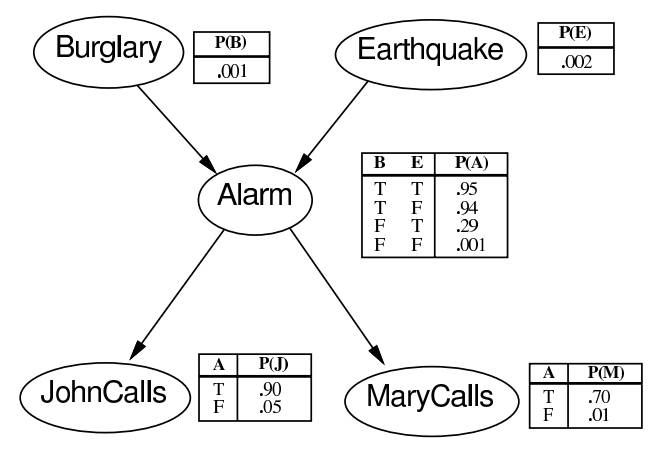
\includegraphics[width=0.86\textwidth]{beliefnet}
    \caption{Belief network for the alarm problem \cite{belfn}}
    \label{fig:beliefnet}
  \end{center}
\end{figure}

Some interesting question we can ask, given this scenario are:

\begin{itemize}
  \item If John calls saying the alarm is ringing but Mary doesn't, what are the
odds it really is ringing?
  \item If the alarm is ringing, was there an earthquake?
  \item What are the chances that both my neighbors call, the alarm is ringing,
but there is neither a burglary nor an earthquake?
\end{itemize}

This last example, for instances, would be calculated as: P(J, M, A, \neg B, \neg E)
= P(J|A) * P(M|A) * P(A|\neg B, \neg E) * P(\neg B) * P(\neg E) =
0.9 * 0.7 * 0.001 * 0.999 * 0.998 = 0.00062.

Notice how counter-intuitive this
example is: the probability of there being an earthquake is about 32 times larger
than there being an earthquake, the alarm ringing and the neighbors calling us,
even if the conditional probabilities are reasonably high (0.95, 0.9 and 0.7).
This is the result of the calculation of the joint probability being an highly
combinatorial problem, which is yet another argument in favor of using PR
rather than subjective heuristics.

\subsubsection{Bayes' and data streams}

In practical ML applications, it is often the case that there is an
incoming stream of new data, rather than one-time batch calculations.
BR can accommodate this way of thinking, which A. Downey called diachronic
interpretation \cite{thbay}, where diachronic means that something is happening
over time (in this case the probability of the hypotheses, as new data arrives).
In order to make sense of this definition, we may rewrite Bayes' rule as:

$$ P(H \mid D) = \frac{P(D \mid H) \, P(H)}{P(D)} $$

Where:

\begin{itemize}
  \item H: hypothesis
  \item D: data
  \item p(H): probability of the hypothesis before the new data is taken into
account. Also called \textbf{prior}. It can either be calculated using background
information or subjectively defined using domain knowledge. Loses significance
as new data is added, so its choice is not determinant to the model's performance
in the long run.
  \item p(H|D): what we want to calculate, the probability of the hypothesis
after considering the new date. It is called \textbf{posterior}.
  \item p(D|H): probability of the data if the hypothesis was true, called
the \textbf{likelihood}.
  \item p(D): probability of the data under any hypothesis, called the
\textbf{normalizing constant}.
\end{itemize}

Under this interpretation, you may continuously feed data into the model and see
the probabilities getting updated. We will see more practical examples of this
in section \ref{sec:pp}.

\subsubsection{Beyond Bayesian Graphical Model}

At first glance, someone who is learning for the first time about PR applied
to ML, may think that graphical models such as the one presented in Figure
\ref{fig:beliefnet} are the best there can be done in terms of using a graphical
interface for solving this kind of problems and that the only thing is missing
is an automated way to make the calculations.

While it is true we have still never mentioned techniques or tools that
automatically do inference over a Bayesian Network, there are several tools
with that capability (including an R package \cite{Hojsgaard2013} or
standalone tools \cite{msbn}).

However, not all PR can be done via Bayesian Networks and not all graphical models
are enough for complete PR \cite{intpp}. PP are the largest class of models available, and there are
also more algorithms for inference than just the calculation of joint
probabilities (like we did in the alarm example), as we will discuss in Section
\ref{sec:pp}.

Bayesian Networks are not the only kind of graphical model. Another one would be
Markov Chains, which is yet another example of a model which is not able to
represent all PR problems. This is clear when we realize that, while PPLs
support numerous distributions (such as Normal, Laplace,
Gamma, Half-Cauchy or \textit{t}), all Bayesian Networks and Markov Chain
can be represented in a PPL by just using Bernoulli distributions \cite{PPm}.
We can see an example of such a translation in Figure \ref{fig:mppl}.

\begin{figure}[t]
  \begin{center}
    \leavevmode
    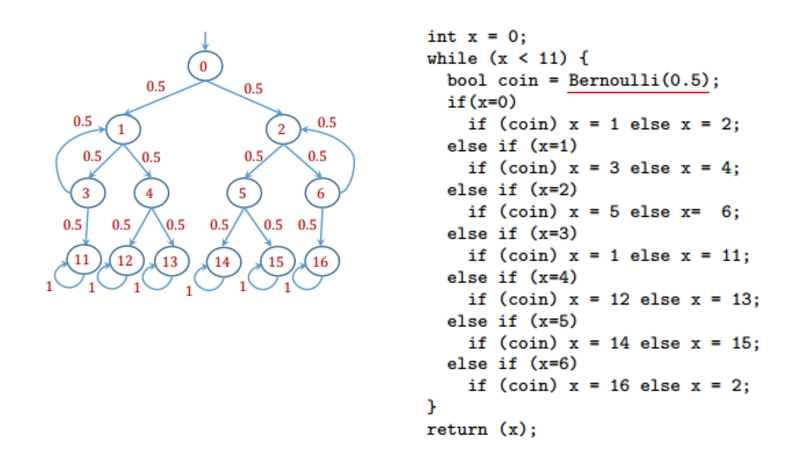
\includegraphics[width=0.86\textwidth]{markppl}
    \caption{Translation of Discrete Time Markov Chain to a PPL \cite{PPm}}
    \label{fig:mppl}
  \end{center}
\end{figure}

% <---- TODO rever com base em prob inference for graphical models

\subsection{Probabilistic Programming Languages}
\label{sec:pp}

\subsubsection{The Probabilistic Program-Model duality}

A probabilistic program (PP) is an ordinary program (that can be written in
mainstream languages such as C, Java or Haskell) whose purpose is to specify
a probability distribution of its variables. This is done by sampling over
several executions of the program. The only needed construct the language
has to support, in order to be able to write a PP, is having a random number
generator \cite{intpp}. This whole concept couldn't be better explained than in this text by Freer and
Roy, regarding Church (a PPL, which we describe in Section \ref{sec:church})
but common to any PP:

\begin{quote}
  ``If we view the semantics of the underlying deterministic language as a map
  from programs to executions of the program, the semantics of a PPL built on it
   will be a map from programs to distributions over executions. When the
   program halts with probability one, this induces a proper distribution over
   return values. Indeed, any computable distribution can be represented as the
   distribution induced by a Church program in this way''~\cite{Freer2012}
\end{quote}

One way to think about this notion is by considering that the program itself
is the model. An example of the relation between a model (expressed in a PPL)
and the implied distribution over its variables (obtained using an inference
method) can be seen in Figure \ref{fig:distribution}, where a variable \textit{flip}
is set to be a Bernoulli distribution and \textit{x} is defined in terms of
\textit{flip}. We can then see how the graphic of the inferred distributions
of \textit{flip's} and \textit{x's} values looks like and confirm what was to
be expected: for \textit{flip's} values lower than 0.5 we see \textit{x} follows
a normal distribution, whereas for values greater than 0.5 it follows a gamma
distribution instead.
 The goal of PP (via PPL) is to enable PR and ML to be accessible to
most programmers and data scientists who have enough domain and programming
knowledge but not enough expertise in probability theory or machine learning.

\begin{figure}[t]
  \begin{center}
    \leavevmode
    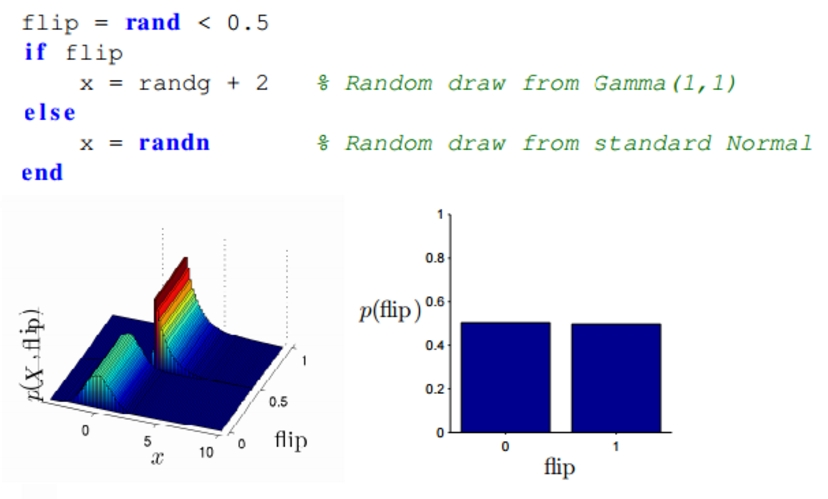
\includegraphics[width=0.86\textwidth]{distribution}
    \caption{Implied distributions over variables \cite{intpp}}
    \label{fig:distribution}
  \end{center}
\end{figure}

\subsubsection{PPLs vs regular PLs}

What is then, a Probabilistic Programming Language (PPL)? First of all, it can
be a standalone language or an extension to a general purpose programming language.
We'll be analyzing examples of languages from either these categories in Section
\ref{sec:art}, but many more exist, such as as Figaro \cite{figaro} (hosted in Scala),
webppl \cite{dippl} (embedded in javascript) or Dimple
\cite{DBLP:journals/corr/abs-1212-2991} (which has both a Java and a MATLAB API).
The key difference between these languages and a PPL is the latter has
the added capability of performing conditioning and inference \cite{Andrieu2003}.

Conditioning is the ability to introduce observations about the real world in
the program. That way, you update the prior probability based
on those observations. Consider the example in Figure \ref{fig:truskill} (which
is a simplified version of how Microsoft applies PP in its Xbox matchmaking
algorithm \cite{minka2012infer}) where the prior is a normal distribution with
equal parameters for all players (shown by the graphic in the top). Then, it
defines how the performance of the player is based on his skill (which at the initial
point in time, is equal to every one of them) and proceeds to make several
observations regarding games between them. Finally, it shows the inferred
probability distribution of the posterior on the bottom graphic.

\begin{figure}[t]
  \begin{center}
    \leavevmode
    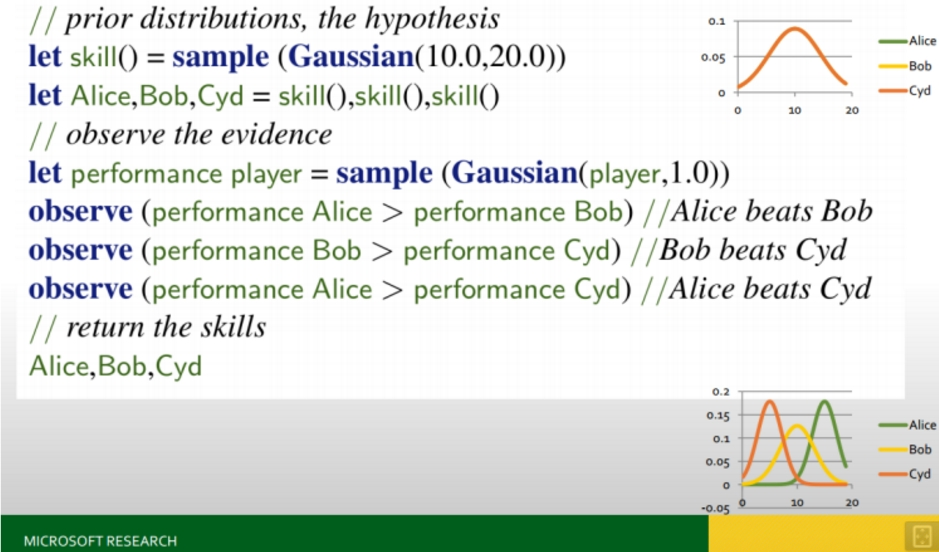
\includegraphics[width=0.86\textwidth]{trueskill}
    \caption{Microsoft Xbox Live True Skill \cite{minka2012infer}}
    \label{fig:truskill}
  \end{center}
\end{figure}

\subsubsection{Inference}

We said that a PPL empowers the user to formalize a model and then query for the
probability distribution of its variables, which is automatically done via
inference. While general-purpose language require you to write one-time
inference methods that tightly coupled to the PP you are inferring on, PPLs
ship with an inference engine suited to most PP programs you can write
\cite{Freer2010}.

An inference engine of a PPL acts similarly to a compiler in a traditional
language: rather than requiring each user to engineer its own, which requires
significant expertise and is a non-trivial and error-prone endeavor, every PPL
has one incorporated.

Having the inference engine work as a separate component, rather than being
tighly coupled to each model, opens up a myriad of new
possibilities mainly in the form of knowledge and tool sharing, as we have
seen in the past in the compiler space. Examples of this would be new
compiler and interpreter techniques (such as working towards scalability or
parallelization), optimizers, profilers or debuggers.

Another great advantage of having a modular inference engine is that we can
try different inference algorithms and pick the one that best fits the problem
at hand. When analyzing which algorithm is more suitable for a certain use case, there are certain
characteristics worth noting \cite{Minka1999}:

\begin{itemize}
  \item Determinism - in equal initial conditions, an algorithm always yields
the same result.
  \item Exact result or approximation.
  \item Guaranteed convergence - an algorithm may or not be guaranteed to reach
a result at some point in time. If not, it's possible that it will run forever.
  \item Efficiency - related to how fast can it reach a result.
\end{itemize}

Microsoft's Infer.NET provides three inference algorithms \cite{msalg}:

\begin{itemize}
  \item Expectation Propagation - deterministic, provides exact solutions only
in some cases, is not guaranteed to converge and is labeled as "reasonably
efficient".
  \item Variational Message Passing - also deterministic, but always gives
approximates results and is guaranteed to converge. It's considered to be the
most efficient of the three for most cases.
  \item Gibbs sampling - non-deterministic, may be able to reach exact result
if given enough time to run, has guaranteed convergence and is regarded as
not-so-efficient as the other two.
\end{itemize}

We can divide the three algorithms into two categories: variational bayesian
methods \cite{Winn2005}\cite{Minka1999} and sampling methods (in the case of Gibbs
sampling, it's based on Markov chain Monte Carlo) \cite{Andrieu2003}. The main
difference, as far as the end-user is concerned, is that variational methods
provide faster results but are subject to bias, whereas sampling methods have
the potential to produce more accurate results (the downside being it's slower
and its convergence is hard to diagnose) \cite{Shen2010}.

Please notice than none of these algorithms provides the same kind of exact
solution as the calculation of the joint probabilities we did in Section
\ref{sec:bayes}. The reason for that is that calculating an exact solution
takes time exponential in the number of variables to run, even if we have smarter
algorithms than the naive calculations we did \cite{Zhang1994}.

\subsubsection{Openbox models}

When compared to traditional machine learning methods (such as random forests, neural
networks or linear regression), which take homogeneous data as input (requiring
the user to separate their domain into different models), probabilistic
programming is used to leverage the data’s original structure. This is done by
empowering the user to write his own models while taking advantage of a re-usable
inference engine. Olivier Grisel called this combination "Openbox models,
blackbox inference engine"\cite{SciPy}.

Rather than using most of his
time performing feature engineering (that is, trying to fit the problem and the
data into an existing model), the user will have the tool necessary to design
the model that best fits the domain he is working on.
Plus, it provides full probability distributions over both the predictions and parameters of the
model, whereas ML methods can mostly only give the user a certain degree of confidence
on the predictions.

\subsection{Conclusion}

Summarizing, PPLs are a step forward in using PR to solve ML problems since
it helps overcome the difficulties in using PR in real world problems. This is
done by adding automated general inference on top of a precise specification
(the program), where in the past models were communicated
using a mix of natural language, pseudo code, and mathematical formulae and solved
using special purpose, one-off inference methods.

This encourages exploration, since
different models require less time to setup and evaluate, and enables sharing
knowledge in the form of best practices and design and development patterns.

However, using a full fledged programming language might still be an entry
barrier. We want to help statisticians and data scientists alike to learn
faster and be more productive using a PPL in a way similar to the tools they
are accustomed to. In order to do so, we'll be combining a PPL with Visual
Programming (Section \ref{sec:vp}).

\section{Visual Programming}
\label{sec:vp}

Visual Programming (VP) can be defined as "any system that allows the user to specify a program in a
two-(or more)-dimensional fashion." \cite{Myers1986}.
In a textual programming language, even though there are two dimensions (one
being the text itself, and the other the optional line-breaking characters),
only one of them has semantics, as the compiler processes text as a
one-dimensional stream.

Examples of systems with additional dimensions are ones that allow the use of
multidimensional objects, the use of spatial relationships, or the use of the
time dimension to specify “before-after” semantic relationships \cite{Burnett1999}.

Research has identified several advantages in the use of VP, such as a natural
way of expressing semantics, good readability, easy interaction, language independence (though
this is not applicable to the work of this thesis, as detailed in \ref{sec:vpe}),
programming at higher levels of abstraction or rapid prototyping \cite{JamalRahmanandWenzel2014},
which is achieved by providing immediate visual feedback \cite{Shu1988}.

The advantages of programming at higher levels of abstraction are known, and
one of them is it exposes users who are not used completely fluent in programming
to a reduced number of concepts \cite{Shu1988}, while decreasing the verbosity of
programs, which can even be useful for seasoned programmers \cite{Myers1990}.
It also reduces the importance of being familiar with syntax, a common cause
of difficulty of adaptation among less experienced programmers when learning
a new language \cite{cunniff1986does}\cite{Carlisle2005}. This difficulty of translating ideas
into syntactically correct statements can also be solved by finding alternative
ways to communicate instructions to the computer \cite{Kelleher2005}.

So, the point of using a VP tool to aid in programming is to overcome the
difficulties that many people have when learning a conventional language
\cite{Lewis1987}. It has been shown this approach can help users without prior, or little,
programming experience to create fairly complex programs \cite{Halbert1984}.
This is specially true within certain small domains, where the language can be
tailored for a subset of tasks rather than trying to be suitable for all kinds
of applications \cite{Kelleher2005}. Tools similar to Excel (spreadsheets) are a prime example of this, where the following
benefits were identified \cite{ambler1987forms}\cite{Lewis1987}:

\begin{itemize}
  \item The graphics on the screen use a familiar, concrete, and visible representation which
directly maps to the user’s natural model of the data
  \item They provide immediate feedback
  \item They supply aggregate and high-level operations
  \item They avoid the notion of variables (all data is visible)
  \item The inner world of computation is suppressed
  \item Each cell typically has a single value throughout the computation
  \item They are non-declarative and typeless
  \item Consistency is automatically maintained
  \item The order of evaluation (flow of control) is entirely derived from the declared cell dependencies
\end{itemize}

Another example of such a domain would be
developing ML applications resorting to probabilistic programming.

Smith and other authors claim that the human thought process is clearly optimized
for multi-dimensional data \cite{smith1977pygmalion}\cite{Clarisse1986},
so all the aforementioned advantages can be explained by how graphical programming is closer
to our mental representation of problems when compared to a textual interface
\cite{Cardellini2002}. As said by Fischer, Giaccardi, Sutcliffe and Mehandjiev:

\begin{quote}
  ``Text-based languages tend to be more complex because the syntax and lexicon
  (terminology) must be learned from scratch, as with any human language.
  Consequently, languages designed specifically for end users represent the
  programmable world as graphical metaphors ... (\textit{such languages aim to}) reduce the cognitive
  burden of learning by shrinking the conceptual distance between actions in
  the real world and programming.'' \cite{G2004}
\end{quote}

This idea as been tested in an empirical study:
in a algorithms course of the United States Air Force academy,
students have consistently shown a preference for solving problems visually,
while it also seems that doing so helped them to achieve better
scores in problem-solving exercises and overperform their colleagues who used
a regular programming language \cite{Cardellini2002}. However, shortcomings of
using VP were also identified, as we will discuss in \ref{sec:crit}.

\subsection{Visual Programming Environment}
\label{sec:vpe}

Boshernitsan proposed a classification scheme for VPLs \cite{Boshernitsan2004}
that divided VPLs in purely visual languages (PVLs), hybrid text and visual systems,
programming-by-example systems, constraint-oriented systems and form-based systems.

In the context of this dissertation, as we want to leverage the advantages of
both a VPL and a PPL while avoiding implementing a PPL, so the obvious choice
is to use an hybrid text and visual system. We will be calling this system a
visual programming environment (VPE). The difference between a VPE and a purely visual language (PVL)
is that, while a PVL is a language \textit{per se} (meaning that it there
is a direct mapping between graphics and execution), VPEs offer a middle ground
between regular textual languages and PVLs: they provide a graphical interface
that can be used to generate code for a target language \cite{Burnett1999}.
An example of a PVL would be MIT's Scratch \cite{resnick2009scratch} and one for
a VPE is the Eclipse IDE plug-in WindowBuilder \cite{winbuild}.

If conceived
correctly, VPEs can help addressing some of the issues raised by critics of VP (detailed in section \ref{sec:crit}),
such as VP's inability to solve real-world large-scale problems. This is done
by applying VP to only subsets of entire systems, making it possible to combine
a general-purpose programming language with the advantages of VP \cite{Burnett1999},
since the code generated by a VPE can be seamlessly integrated in any project
built with its target language.

Concretely, VPEs are able to overcome the tradeoff of control for simplicity
commonly made by VPLs: even if a certain idiom cannot be represented by its
graphical form, the user can later edit the generated code to include it. This
makes it possible to design scalable programs, both in terms of performance
(since the user can still access all the target language's low-level features) and development
(because all the advantages of programming visually are still present).

\subsection{Visual Dataflow Programming}

A Dataflow Programming Language (DPL) is built upon the notion that data flows
from one node to another. Therefore, in this paradigm a program is internally
represented as a direct graph \cite{Hils1992}. This graph is constituted by
three kinds of nodes (also called blocks): sources (take no input and produce
output), processing/transformation (take an input and produce an output based
on it) and sinks (only take input and don't produce output) \cite{Sousa2012}.

The edges behave like unbounded in-order queues and define the data dependencies
between nodes \cite{Johnston2004}, connecting input ports to output ports. Nodes process data asynchronously, as soon
as all of its inputs are available. There are at least two ways a dataflow program
can operate: either from left to right (from higher topological order to lower,
also called data-driven or push-based) or right to left (in inverse topological order, called
demand driven or pull-based) \cite{Johnston2004}.

Some authors have identified features which are important in a DPL
\cite{ackerman1982data}\cite{wail1995can}:

\begin{itemize}
  \item Freedom from side-effects: a block can't do more than producing an
output based on inputs, being it I/O or variable re-assignment, for instances.
  \item Locality of effect: this means having well-defined and small scopes. A
variable should not be used in more than one block (the one it is connected) to
via input port.
  \item Data dependencies equivalent to scheduling: there is no notion
of time in a DPL. However, a block will only run as soon as its inputs are ready,
creating an implicit scheduling.
  \item Lack of history sensitivity in procedures: no global variables. A node
can only access its input ports.
\end{itemize}

Looking at these features, the reader can realize that in a language where all
these rules are followed it is also possible to achieve implicit concurrency.
Meaning that, once a program is specified, the user gets out-of-the-box concurrency
without manually having to program it \cite{Sousa2012}.

As we will see in \ref{sec:art}, there are several VPL and VPE that resort to the
dataflow paradigm. This could be explained by how easily DPL map to
a visual representation \cite{Johnston2004}. This kind of tool can be described
as Visual Dataflow Programming (VDP).

VDP shares the same challenges as other VP paradigms: achieve the right level
of granularity (abstract neither too much so that the users can't express everything
he needs to nor too little, making the representation as complex as its textual
counterpart).

A big challenge in VDP that is not present in other VPL paradigms
is not how to transpose the dataflow graph to a graphical
representation but rather representing control flow semantics within dataflow
\cite{Cox2011}. Several solutions have been proposed, some of which violate
the pure DFP principles by not being completely stateless while others introduce
cycles in the graph \cite{Mosconi2000}.

\subsection{Evaluation}
\label{sec:eval}

Even if the goals of VP are clear (to make programming more understandable, ensure
correction and be faster to develop in) the best way to achieve them is still a matter of
discussion. Like in the design of any programming language, there are some
best practices to guide the design of a VPL, some of which have been identified
by Burnett \cite{Burnett1999} and are listed below.

\begin{itemize}
  \item Concreteness - it's opposite of abstractness. The program express values
and instances of values rather than meta-information such as types or classes.
  \item Directness - work with concrete values rather than possible ones.
  \item Explicitness - everything that there is to be known about the program
can be easily understood by looking at the graphical representation, the
user does not need to infer semantics by himself.
  \item Immediate visual feedback - every change to the program should be
immediately propagate to change in the affected output. Spreadsheets are an example of
this.
\end{itemize}

However, these are just guidelines and do not guarantee the efficacy of a VPL.
Some VPEs sacrifice some of these principles for the sake of completeness:
Viskell (described in \ref{sec:viskell}) violates directness by allowing to
work with the option monad, or concreteness by placing a great emphasis on type
definition.

Whitley and Blackwell \cite{Whitley1997} said that, because the design decisions
in a VPL lack formal basis, the only way to assess if they really contribute
to facilitate the programmer's cognitive processes while programming is through
empirical studies. In their studies, they have found that while subjects
cited ease of learning as a benefit of VPLs, their opinions differed when asked
if using a VPL had a positive impact in productivity during a project.

They also claim that there is a gap between academia and industry programmers.
In contrast to the first group who tends to focus on theories of cognition to justify the use
of VPL, the second is more interested in potential improvements in "potential
improvements in productivity that arise from straightforward usability issues".

Some metrics that can be taken into account when assessing a VPL's efficacy
are learning time, execution speed and retention \cite{Myers1990}.

\subsection{Criticism}
\label{sec:crit}

In this section, we'll be trying to summarize some of the criticism made to VP,
while proposing solutions to some of the issues mentioned and discard some of
the others as non-applicable in the context of this thesis.

There are people who claim VPLs lack visual abstraction mechanisms that are as effective
as those offered by text-based languages, so they are not well-suited to develop
large applications \cite{JamalRahmanandWenzel2014}. Some of the techniques
currently used in real-world software development include iterative design and
interactive prototyping, two principles that are promoted by the usage of VPLs.
Also, it has been shown that the richness of the visual paradigm
introduces new ways of approaching programming problems, particularly for
those not trained in traditional software development methods \cite{JamalRahmanandWenzel2014}
(such as data scientists, which constitute the target audience of this work).
Studies also shown that fairly complicated algorithms, such as garbage collection,
could be described graphically \cite{Myers1990}.

Green also discusses, contrary to some other evidence we discussed before \cite{Cardellini2002}\cite{Burnett1999},
how lab studies failed to collect evidence in favor of the productivity gain of
VPLs, even though he admits users like and use them \cite{Shu1988}. He also points
how that VP systems "do nothing that can’t be done as well or better with straight text"
and identifies the real issues as "how layout and locality can be used to convey meaning".
According to our definition of VP, every system that allows the user to express
himself in more than one dimension (such as using layout and locality, as proposed
by Green), so it seems that the proposed alternative could be a VPL.

In his \textit{"No silver bullet - essence and accidents of software engineering"} paper, Brooks
says that \textit{"A favorite subject for PhD dissertations in software engineering is graphical, or visual,
programming—the application of computer graphics to software design ...
Nothing even convincing, much less exciting, has yet emerged from such efforts. I am persuaded that nothing will. In
the first place, ... the flowchart is a very poor abstraction of software structure....
It has proved to be useless as a design tool.... Second, the screens of today are too small, in pixels, to show both
the scope and the resolution of any seriously detailed software diagram.... More fundamentally, ...
software is very difficult to visualize."} \cite{Brooks1986}. While one may be tempted
to be convinced by Brooks' initial rhetoric, what he wrote does not seem to apply
to the work of this thesis because: a) we won't be using executable flowcharts,
but rather a dataflow VPE approach, as described in \ref{sec:vpe} and b) as time passes screens
are getting bigger and with higher resolutions, a low-end screen by today's standards
would be state of the art in 1986, when Brooks wrote that. The final claim that
software is hard to visualize, backed by Dijkstra's letter where he states that
\textit{"I was recently exposed to ... what ... pretended to be educational software for an introductory programming course.
With its ‘‘visualizations’’ on the screen, it was ... an obvious case of curriculum
infantilization ... We must expect from that system permanent mental damage for most students
exposed to it."} \cite{dijkstra1989cruelty}, is contrary to many studies done in cognitive science
\cite{Lewis1987}\cite{cunniff1986does}\cite{Carlisle2005}.

Myers admitted that the key for a successful application of VP to a real-world
problem was to identify "appropriate domains and new domains to apply these
technologies to" while recognizing that we have already witnessed how VP can help
non-programmers work in limited domains \cite{Myers1990}.

We do believe that
data mining can be one of those domains (as shown by the popularity of RapidMiner) \cite{kdn},
so it would make sense to extend the current state of the art with a tool that
combines VP and PP. This view is aligned with Burnett's claims that VP makes
programming easier for specific audiences \cite{Burnett1999}. It is also our belief
that, by only applying VP to a specific part of a larger system (in this case,
the ML module that uses PP) we can overcome the problems that usually arise when
scaling up VPL \cite{Burnett1995}; successful examples of such an approach
include the design of GUIs via a VPE (such as WindowBuiler \cite{winbuild} or
the Android Studio's layout editor \cite{layouted}).

Myers also identified some of the problems that are yet to be solved
regarding VP \cite{Myers1990}:

\begin{itemize}
  \item \textbf{Difficulty with large programs or large data}. Almost all visual representations are physi-
cally larger than the text they replace, so there is often a problem that too little will fit on
the screen.

We intend to solve this issue by studying the application of some techniques
that provide a greater level of abstraction in order to be able to transmit
more semantics while avoiding the layout to get cluttered with details \cite{Burnett1995}.
  \item \textbf{Poor representations}. Programs are hard to understand once created and
difficult to debug and edit. The larger the size, the worse this problems becomes.

This is related with the previous point and the proposed solution is similar.
  \item \textbf{Need for automatic layout}. When a program gets too large the layout
becomes too hard to manage, a single addition of a piece may oblige the user
to move a great number of blocks in order to avoid collisions and preserve
readability. One way to deal with this would be to automatically generate an
attractive layout.

This problem is out of the scope of this thesis, although
it certainly seems important for the future of VPL.
  \item \textbf{Lack of formal specification}. Currently, there is no formal way to describe
a VPL such as the Backus-Naur Form, even if there is some work towards one was
already been made \cite{selker1988elements}.

Again, this is out of scope, even
if we will make an attempt to specify a grammar that defines the boundaries of
what would be a valid graph.
  \item \textbf{Lack of Portability of Programs}. A program written in a textual language
is as portable as a text file but VPLs require special software to view and edit.

While the implementation of the VPE's frontend to be done in this thesis is still a matter
of study and is undecided, there is the possibility of building one using the
HTML/CSS/javascript stack, making it portable across browsers for view and edition.
It is also our aim to provide an intermediate representation in a data-representation
format such as JSON or XML, so that a program built in a certain frontend can
be processed by any other.
  \item \textbf{Tremendous difficulty in building editors and environments}.
In 1990, each graphical language required its own editor and environment, and there were no general purpose
VPL editors.

Currently there are alternatives of re-usable frontends for VPLs,
such as Blockly \cite{blockly} or GoJS \cite{gojs}.
  \item \textbf{Lack of evidence of VPLs' worth}.

This issue was discussed in section
\ref{sec:eval}, and we conclude that within certain domains (such as VP applied
to PP) and target users (inexperienced programmers), there may be benefits in
productivity when using a VPE.
\end{itemize}

Another question that arises is how to represent and manipulate arrays. In the
empirical study made by the creators of RAPTOR, students performed statistically
significantly worse on the array question when using a VPL \cite{Cardellini2002}.
This is something to consider in the future, to investigate if handling arrays
functionally (by considering them as immutable values where common functions over
iterable data structures could be performed, such as map, filter and reduce)
could improve users' usage of the VPL.

One of the concerns of another empirical study's respondents was that high-level VPLs might deny
them access to the low-level facilities of the machine that are so important in PC programming \cite{Whitley1997}
but, as stated before, this problem is alleviated (if not completely eliminated)
by using a VPE rather than a purely visual VPL, since the user can later
edit the generated code, where he has access to all the language's features.

\section{State of the Art}
\label{sec:art}

The purpose of this section is to try giving an overview over the existing tools
currently used in either VP (purely visual VPLs or VPEs) or PPLs.

\subsection{PPLs}
\label{sec:ppls}

There is a great number of PPLs, so our criteria to pick which of them to analyze
was popularity, which we assessed based on a rough estimate of the number of papers
that referenced each language.
At the same time, we tried to pick languages from different
ends of the spectrum: functional/imperative/object-oriented, statically/dynamically
typed, one that runs in the JVM, one from the .NET stack and another one written
in javascript which runs in the browser.

One advantage of the languages that do not require compilation
(such as WebPPL or Church) is that we can display results to the user faster and
without having to re-compile every time we change
the model, making it as close to immediate visual feedback as possible.

The way we're planning to validate this thesis hypothesis is by converting
models in the literature from a textual form to a graphical one (more on this in
section \ref{chap:chap3}), so having
a reasonable amount of models in a given language acts as an incentive to use
it as a target for code generation in the tool we'll develop.

\subsubsection{WebPPL}
\label{sec:webppl}

WebPPL was written as part of a course on PP and inference in PPLs \cite{dippl}.
Therefore it serves more as an educational tool rather than a language that aims
to be production-ready, despite including several inference algorithms (such as
MCMC and variational ones). It is hosted in javascript, meaning that it extends
the language's capabilities and is totally cross-compatible; in short, it acts
as a library.

Its main advantage and the reason why it would be interesting
to be the target of our tool is that, because it is written in javascript, it runs
in the browser without having to be ran externally, reducing the time between
designing and getting visual feedback.

\subsubsection{Church}
\label{sec:church}

We started by looking into Church because it is based on pure Lisp (therefore
it is also based on lambda calculus and purely functional programming) \cite{Goodman2008} and believed it could
be more expressible (in the sense that we could express equally complex models
with less code) than its non-functional counterparts. While maintaining the same Lisp-like syntax,
it also has an implementation in javascript called webchurch \cite{church},
with all the associated advantages (described in \ref{sec:webppl}).

The Church language is being replaced by VentureScript, a language that is part
of the Venture platform for PP and that can be written both in a Church or javascript-like
syntax \cite{probcomp}. Having been written by the same authors as WebPPL but
with the purpose of being used to solve real problems instead of just acting as
an educational tool, if we were to choose a PPL hosted in javascript to support
in our tool, the natural choice would be VentureScript.

\subsubsection{Infer.NET}

Infer.NET is being developed by Microsoft Research Cambridge and intends to
empower .NET languages (not only C\#, but all languages in the stack, including
F\#, Visual Basic and Iron Python) with PP capabilities \cite{InferNET14}.

Similarly to C\#, it requires a compile step and is statically typed. Unlike
Church/VentureScript, it cannot represent all kinds of PR models, as it fails to handle
non-parametric models.

It has several advantages
that make it a prime candidate to be the target of this dissertation: extensive
documentation (not only a reference manual of the API), several examples with
various levels of complexity (which is very useful for our hypothesis validation's
process) and an active community, with the contributors
actively participating in a discussion forum and available to clear any doubts
users might have. These reasons, as well as being part of the popular .NET
stack, make Infer.NET a strong candidate to be used as the target language of our tool.

\subsubsection{Figaro}

Figaro is similar to Infer.NET: a statically typed language that requires compilation
and runs a popular environment (in this case, the JVM, since Figaro is hosted in
Scala) \cite{figarot}. It is used by Charles River Analytics in production, so
in spite of being still under development it seems to be useful for end-users and
is not restricted to research groups.

Unlike Infer.NET, it can represent arbitrary models without restrictions, but
examples using the language are scarce so using at as a basis for the thesis
would require extra work converting examples from other languages to Figaro
before developing them in a graphical manner.

\subsection{Tools using VDP}
\label{sec:sotavdp}

\subsubsection{NoFlo}
\label{sec:noflo}

NoFlo is a visual open-source implementation in JavaScript of Flow-Based Programming \cite{noflo}
(which is a form of dataflow programming) and was designed for general-purpose
programming, even if it is more suitable for web programming (being written in
JavaScript it has easy access to DOM manipulation capabilities), there are
examples of it even being used for controlling a drone.

\begin{figure}[t]
  \begin{center}
    \leavevmode
    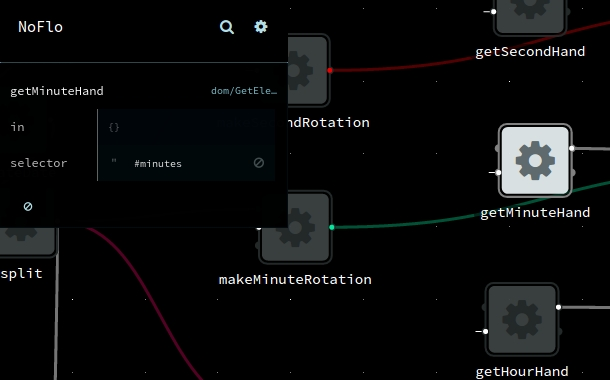
\includegraphics[width=0.86\textwidth]{noflo}
    \caption{Example of node expansion in NoFlo \cite{noflo}}
    \label{fig:noflo}
  \end{center}
\end{figure}

\begin{figure}[t]
  \begin{center}
    \leavevmode
    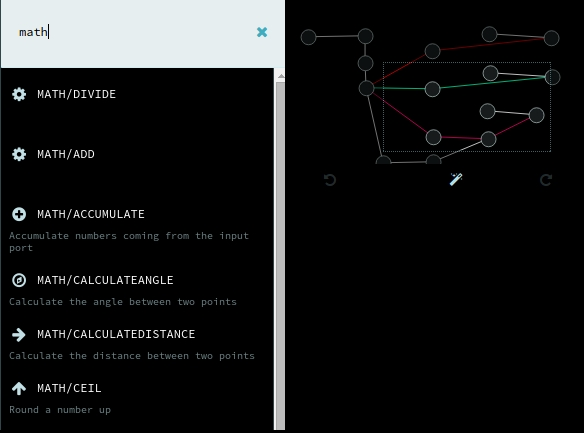
\includegraphics[width=0.86\textwidth]{noflo2}
    \caption{NoFlo node search and minimap navigator \cite{noflo}}
    \label{fig:noflo2}
  \end{center}
\end{figure}

From experimenting with the tool, we found some characteristics that serve as a
lesson of what works well and what doesn't:

\begin{itemize}
  \item A node has the least information possible, yet it can be clicked to
show details, such as some usage notes or seeing some inputs or parameters.
An example of a common NoFlo layout with a node expanded can be seen in Figure
\ref{fig:noflo}. This contributes to saving space in the layout while maintaining
flexibility.
  \item You can search for a block by its name (see Figure \ref{fig:noflo2}).
  \item There is a minimap that helps to navigate the screen, so we can have
a higher level view of the layout \ref{fig:noflo2}).
  \item Weak typing makes it confuse to use some of the nodes, it is unclear
when we can connect input and outputs with mismatching labels, because sometimes
they are compatible and other times they aren't.
  \item Sometimes errors appear immediately, others we can just see them in
runtime. This would be fine as long as it was clear that there was an error,
but that is not the case because the messages blend in with the UI and are
not easily noticeable.
  \item When choosing new blocks, it is often hard to understand what is their
functionality because most nodes have no description other than their name.
  \item Blocks have icons, which presumably provide some visual information
about their functionality (see Figure \ref{fig:noflo2}), but is hard to
understand what the difference between the various icons is. What seems to be a
good idea, to have icons in blocks to identify them by functionality, as the
opposite effect and negatively affects usability.
\end{itemize}

The last four items can convince the reader of the following conclusion: in VPLs, explicit
is better than implicit. Clarity can undoubtedly make all the
difference between a language that can be intuitively used and one that, despite
all its virtues, could take some more time to master.

\subsubsection{RapidMiner}

According to the popular data mining portal KDnuggets' latest tool popularity
poll \cite{kdn}, RapidMiner is the most popular visual tool to use in applied
machine learning. It is also the most complete, featuring 1500 different blocks \cite{rapidminer}.

The product has too many features to be able to deeply analyze each one of them,
including cloud and repository capabilities for storing and sharing work,
mechanisms for deploying models developed locally to a production server or
an API for developing new blocks. RapidMiner is actually more of a suite rather
than just a tool, so in our analysis we'll restrict ourselves to the design of
a model.

The most differentiating factor between RapidMiner and the other VPLs we studied
is that it splits its view between process and results. In the first one, the
user can design the model and then he must run it and go to results to see the output.
Even if goes against the principle of providing immediate feedback to the user
advocated by some VPLs' designers (as discussed in \ref{sec:vp}), it does seem to make
sense in its use case. The reason for that is that production machine learning applications
running batch jobs can take a reasonable amount of time to run, and the analysis
of its results before changing the model can also take some time. This is
different from people using 3D editors (like Blender), where they the trial and
error cycle is much shorter, and users need to get feedback about their changes
much more often.

Having no need to be continuously looking at the output reduces the importance
of it being shown in the same space as the program we're designing, and we can
save space in the layout by moving it to a different tab. On the other hand,
RapidMiner is flexible enough that allows the user to place both the process
and the results windows side by side, so it really is up to the user to decide
how important is it to be seeing everything at the same time. A tool which doesn't
support moving windows and tabs must make a choice whether or not to have the
output shown alongside with the program.

Other strengths of RapidMiner include having error indicators in each block
and thorough descriptions of each
node's functionality, input, output and parameters, including examples. It also
provides visual clues about a node's functionality by using not only meaningful
icons but also colors. This can be observer in Figure \ref{fig:rapidminer},
where file reading nodes are gray, model-related ones green and those related
with data preparation are in pink.

\begin{figure}[t]
  \begin{center}
    \leavevmode
    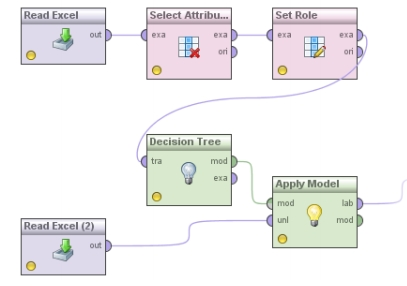
\includegraphics[width=0.86\textwidth]{rapidminer}
    \caption{Classifier in Rapidminer \cite{rapidminer}}
    \label{fig:rapidminer}
  \end{center}
\end{figure}

Something that doesn't seem to work particularly well for someone using the tool
for the first time are the abbreviated labels in the ports. They are cryptic
enough that an inexperienced user has to click the node and read the description
to understand what they are. Maybe it would make sense to either write the full
label for the sake of clarity, or just don't show anything at all.

\subsubsection{Weka Knowledge Flow}

Weka Knowledge Flow is one of the available frontends (others being APIs and a GUI Explorer)
to WEKA's core algorithms \cite{weka}.

\begin{figure}[t]
  \begin{center}
    \leavevmode
    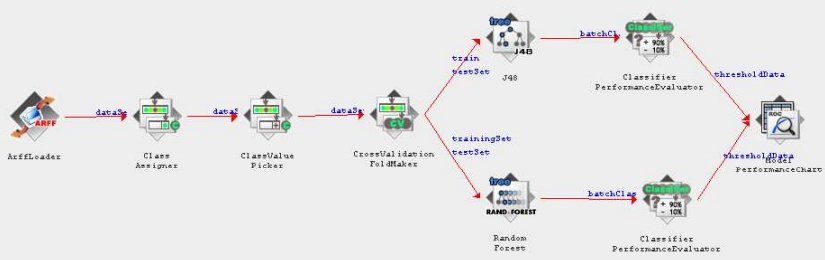
\includegraphics[width=0.86\textwidth]{weka}
    \caption{ROC curve in Weka Knowledge Flow \cite{weka}}
    \label{fig:weka}
  \end{center}
\end{figure}

In this tool, inputs are not connected to specific ports, but rather to a block.
The semantics of the connection is expressed on the edge's label. This can save
some space in the layout as the nodes can be smaller, but in order to understand
a node's input, the user has to waste time following all the edges backwards
until he finds the label, which doesn't seem a reasonable tradeoff.

Weka Knowledge makes a good use of icons to differentiate between different node
types. Not only is it easy to the user to distinguish between source, processing
and sink nodes, but also between the different processing nodes' categories
(such as filters, classifiers and clusterers).

\subsubsection{Blender Composite Nodes}

Blender Composite Nodes is part of the Blender open-source 3D computer graphics
software and provides a way for the user to visually build (through a dataflow
representation) a script that can be applied to images or Blender scenes \cite{blender}.

It incorporates common VDP idioms such as source nodes (such as render layers or
RGB), processing nodes (where you can apply blur, shift an RGB curve, etc) and
sink nodes (it's the way to finalize a script and save, or display, the result).
It is interesting to note that
Blender Composite Nodes does not incorporate processing nodes with filter semantics
\footnote{We mean by filter that the result is a subset of the input. Blender has
graphical filters, which are analogous to a functional map operation.},
which is an example of a VPL that intentionally did not incorporate a common
idiom in VDP because it does not make sense for its domain.

\begin{figure}[t]
  \begin{center}
    \leavevmode
    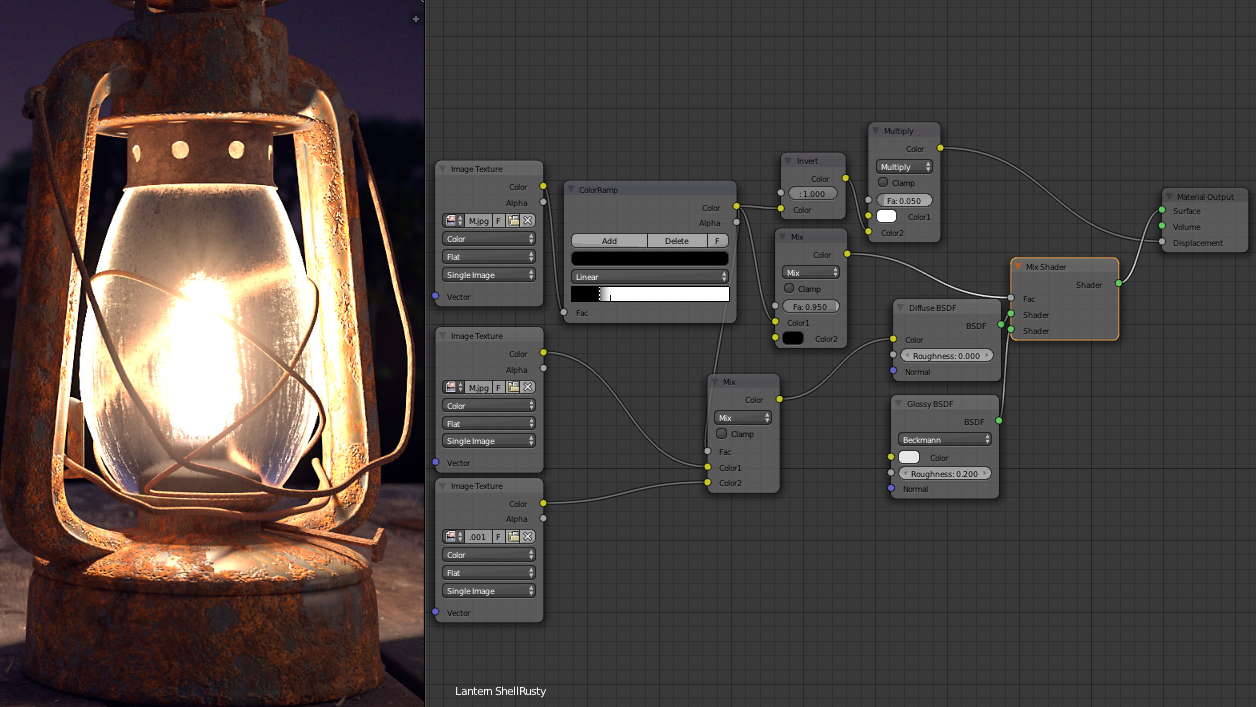
\includegraphics[width=0.86\textwidth]{blender}
    \caption{Script for texture transformation in Blender \cite{blender}}
    \label{fig:blender}
  \end{center}
\end{figure}

There are several interesting characteristics that are worthy highlighting:
\begin{itemize}
  \item Composite Nodes assigns a color to each type, so that the user can
easily understand the type of each input or output (see Fig. \ref{fig:blender}).
  \item Implicit conversions for some of the types. For instances,
a conversion from a vector (which are always three-dimensional) to a value yields
the mean of the vector's elements. In figure \ref{fig:blender} we can see that
some values are connected to a different type (among others, the first input
node's color is connected to a simple value named 'Fac'), which is valid behavior.
  \item Incorporating a custom interface within each node. This helps to reduce
the space occupied by the program, since there is no need to create inputs for
every single input in a processing node. It also simplifies the VPL's usage,
because since some types can only exist within certain nodes, and by not being
able to instantiate them outside those nodes, we reduce the possible choices
for input nodes. An example would be the image type enumeration, that we can
see in figure's \ref{fig:blender} input nodes.
  \item Node groups which are essentially an encapsulation
of a set of nodes, resulting in another node that can be re-used, help the user
create his own set of abstractions. Our texture transformation example could
be saved into a node group, so that we can use it in another script without
needing to copy everything from one place to the other or cluttering the new
script's interface with several new nodes. The concept is analogous to functions
in programming.
\end{itemize}

\subsection{VPEs}

In this section we'll be describing three visual programming environments. By VPEs
we mean tools where the user can express the program in a graphical manner that will
later be translated into valid code, regardless of it being executable directly
on the VPE or not.

\subsubsection{Blockly}

Blockly is more than a VPE, it actually is a library for building VPEs \cite{blockly}.
It is fully open source, runs on the browser (in a fully client-side manner) and
was developed to be extensible.

Blockly does not adopt the VDP paradigm, it instead uses a system of blocks
similar to a puzzle, as you can see in Figure \ref{fig:blockly}.
Another useful feature is basic type checking,
so that users can't connect blocks that wouldn't make sense, such as applying an
uppercase function to a number. The way Blockly is built, it is possible to stop the user
from producing an invalid program.

\begin{figure}[t]
  \begin{center}
    \leavevmode
    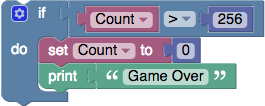
\includegraphics[width=0.86\textwidth]{blockly}
    \caption{Blockly example \cite{blockly}}
    \label{fig:blockly}
  \end{center}
\end{figure}

According to its authors, the reason why they didn't choose to adopt VDP is that
they believe the generated code doesn't look like the VDP graph, making it harder
from a user who later transitions from the tool to textual programming to adapt
to the new format.

It is possible to define new blocks as well completely controlling
how generated code will look like, as well as defining new types. These features
seem to be enough that Blockly can be considered a framework complete enough to
be suitable for building most VPEs and, because it is open-source, it can be
unlimitedly extended.

\subsubsection{Viskell}
\label{sec:viskell}

Viskell is \textit{"an experimental visual programming environment for a typed
(Haskell-like) functional programming language"} \cite{viskell}. Its authors
assume their main goals are, among others, to create a readable and compact
visualizations for functional programming and addressing the scalability issues
of larger visual programs. They state that, in order to achieve the latter goal
and being able to scale up, Viskell should combine a simple core language with
a good type system.

This VPL does not resemble the most popular ones, having some main differences:
the program is designed from top to bottom rather than left to right, blocks
don't have icons but explicit names and all ports have explicit types. This class
of design choices don't seem to be clearly superior to other state of the art tools,
so probably we won't be including them in our VPE.

\begin{figure}[t]
  \begin{center}
    \leavevmode
    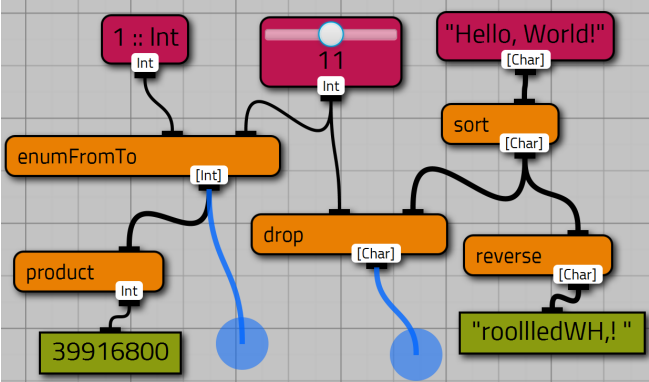
\includegraphics[width=0.86\textwidth]{viskell}
    \caption{Viskell example \cite{viskell}}
    \label{fig:viskell}
  \end{center}
\end{figure}

Nevertheless, there are other interesting features in Viskell, many of which
are tightly coupled to functional programming (such as how it supports currying,
anonymous functions or case expressions). The exception is the capability to
have an incomplete graph and allowing the user to textually insert code to fill
in the gaps (see the blue areas in Figure \ref{fig:viskell}).

Being a work in progress, its authors have pointed out ideas of how to deal with
increased program complexity that they have still not implemented in the language.
Some of them are shown in Figure \ref{fig:viskell2} and outlined below:

\begin{itemize}
  \item Vertical composition of blocks: in the example it is extensively used
in the last ("concatMap") block.
  \item Inline display of constants: as seen in the first block "enumFrom",
where 1 is written inline rather than being a separate source block. It is a form
of horizontal composition.
  \item Functions as constants to higher order functions: represented by the
right-hand side of the 3 blocks in the middle ("map", "groupOn" and "concatMap").
\end{itemize}

This way, we eliminated most of the connections between nodes and achieved a
more compact (we have 4 arcs in a representation that would use more than 20 in
its original format) and readable representation.

\begin{figure}[t]
  \begin{center}
    \leavevmode
    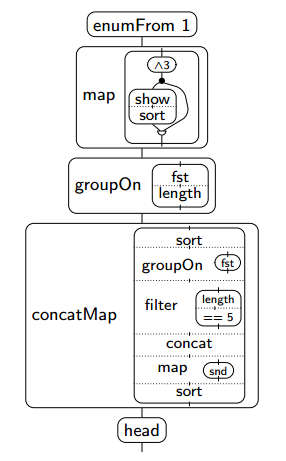
\includegraphics[width=0.86\textwidth]{viskell2}
    \caption{Compressed visual representation example \cite{viskell}}
    \label{fig:viskell2}
  \end{center}
\end{figure}

\subsubsection{WindowBuilder}
\label{sec:winb}

One domain where VPLs have been successfully applied is UI design. Instead of
going through the tedious task of writing boilerplate code (often having to
memorize complicated function signatures) and needing to memorize APIs, users
can just drag and drop elements on the screen.

The Eclipse IDE provides several plugins on its marketplace, one of which is the
WindowBuiler plugin \cite{winbuild} to build Java SWT/Swing UIs.

WindowBuilder is a bi-directional and WISIWIG tool (What You See Is What You Get), meaning
that it generates code that faithfully represents the drawn UI and it is also possible to
directly edit the code and see the updated result back in the design view.

Since defining UIs is a very different domain from PP there are not many features
that we can use from WindowBuilder in our future VPE. The exception is the
bi-directionality of code, which could be useful in certain scenarios.

\begin{figure}[t]
  \begin{center}
    \leavevmode
    \includegraphics[width=0.86\textwidth]{winbuild}
    \caption{WindowBuilder's design view \cite{winbuild}}
    \label{fig:winbuild}
  \end{center}
\end{figure}

\subsection{VIBES}
\label{sec:vibes}

VIBES is a tool, developed by John Winn during his PhD, that allows variational
inference to be performed automatically on a Bayesian network \cite{Winn2005}
defined graphically.
It was written to serve as proof of concept for the variational message passing (VMP)
algorithm, so it has reduced focus on human-computer interaction. Other than its representation
of deterministic inputs with a different edge style than undeterministic ones and
usage of plates to represent loops, from a usability point of view it's not very interesting.

\begin{figure}[t]
  \begin{center}
    \leavevmode
    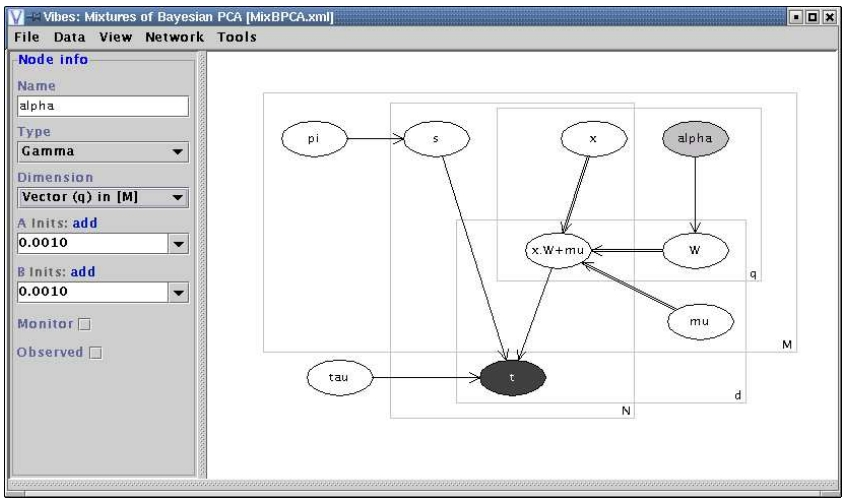
\includegraphics[width=0.86\textwidth]{vibes}
    \caption{Example of a model using VIBES \cite{Winn2005}}
    \label{fig:vibes}
  \end{center}
\end{figure}

\subsection{WinBUGS}
\label{sec:wbugs}

Similarly to VIBES (described in \ref{sec:vibes}), WinBUGS is a framework with a graphical
component which s part of the Bayesian inference Using Gibbs Sampling (BUGS) project.
It allows the user to, graphically or textually, define a model and automatically perform inference
on it (unlike VIBES, the inference algorithm is Gibbs sampling, a method that
resorts to a Markov chain Monte Carlo technique) \cite{Lunn2000}.
Its interface is very similar to VIBES and the only difference between them,
besides the algorithm used, is that WinBUGS provides a bi-directional conversion
between graphical and textual representations.

\begin{figure}[t]
  \begin{center}
    \leavevmode
    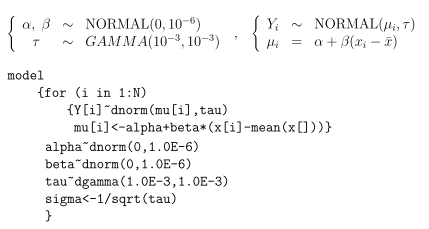
\includegraphics[width=0.86\textwidth]{winbugs}
    \caption{Example of a model translated to WinBUGS textual form \cite{winbugs}}
    \label{fig:winbugs}
  \end{center}
\end{figure}

In Figure \ref{fig:winbugs}, we can see that WinBUG's textual representation of
a simple model can already be harder to understand than the mathematical
formalism it represents. This is exactly the problem we want think it can be
solved with a proper VPE.

\section{Conclusions}

In this section we have seen the application of VP concepts to tools, confirming
the usefulness of many of the concepts studied in the Secton \ref{sec:vp}.

By comparing the different VP applications, we have identified useful features
such as the use of color and icons to transmit meaning, block compression (either
hiding block details or even the grouping of several blocks in different manners),
zooming in and out, minimap navigation, explicit errors, bi-directionality (
being able not only to convert graphics to code, but also vice-versa) and strong typing.

Equally useful to knowing what features are useful is to understand which pitfalls
to avoid, such as not including labels or icons for the sake of having a simpler
interface, resulting being an interface where semantics are too implicit and
hard to capture quickly. One of main goals is to avoid having a VPL that is harder to understand
than the original representation of the model we are developing, similarly to
what happens with WinBUGS textual representation.
